\documentclass[11pt,a4paper]{article}
\usepackage[margin=1.5cm]{geometry}
\usepackage{graphicx}
\usepackage{booktabs}
\usepackage{amsmath,amssymb}
\usepackage{subcaption}
\usepackage{hyperref}
\usepackage{microtype}
\usepackage{siunitx}

\hypersetup{
    colorlinks=true,
    linkcolor=blue,
    citecolor=blue,
    urlcolor=blue
}

\graphicspath{{figures/}{../22pade/}}

\pagestyle{plain}

\begin{document}
Shaded bands indicate Jackknife envelope uncertainty, and solid lines denote mean parameter fits.
\begin{figure}[htbp]
    \centering
    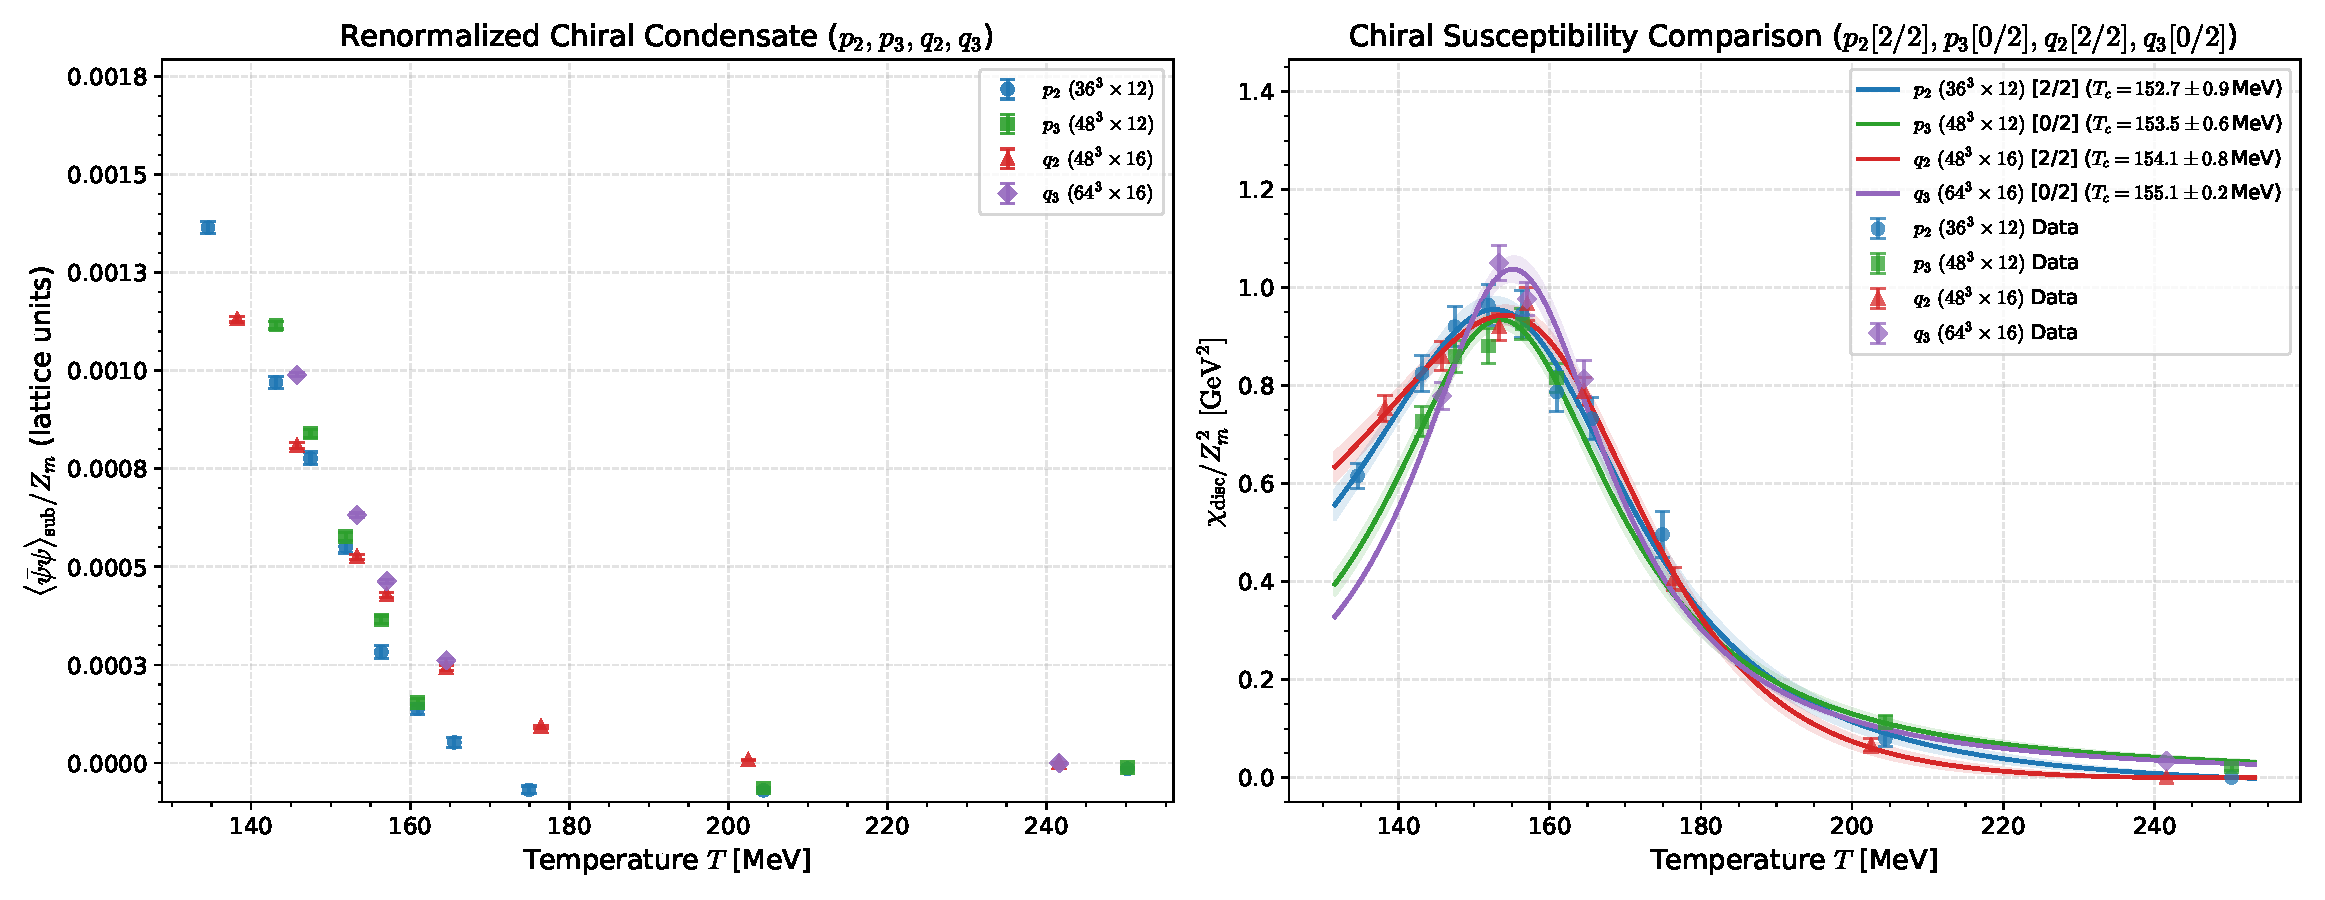
\includegraphics[width=\textwidth]{figures/chiral_lcp_comparison_p2_22_p3_02_q2_22_q3_02.pdf}
    \caption{Renormalized chiral condensate $\langle\bar{\psi}\psi\rangle_{\rm sub}/Z_m$ in lattice units (left) and renormalized chiral susceptibility $\chi_{\mathrm{disc}}/Z_m^2\,[\mathrm{GeV}^2]$ (right) comparison across all four LCP ensembles with Padé configuration: $p_2\,[2/2]$, $p_3\,[0/2]$, $q_2\,[2/2]$, and $q_3\,[0/2]$. }
    \label{fig:combined_p3_02_q3_02}
\end{figure}

The value of condensation in high temperature maybe negative , light condensate decrease much faster than the strange condensate. 

\begin{figure}[htbp]
    \centering
    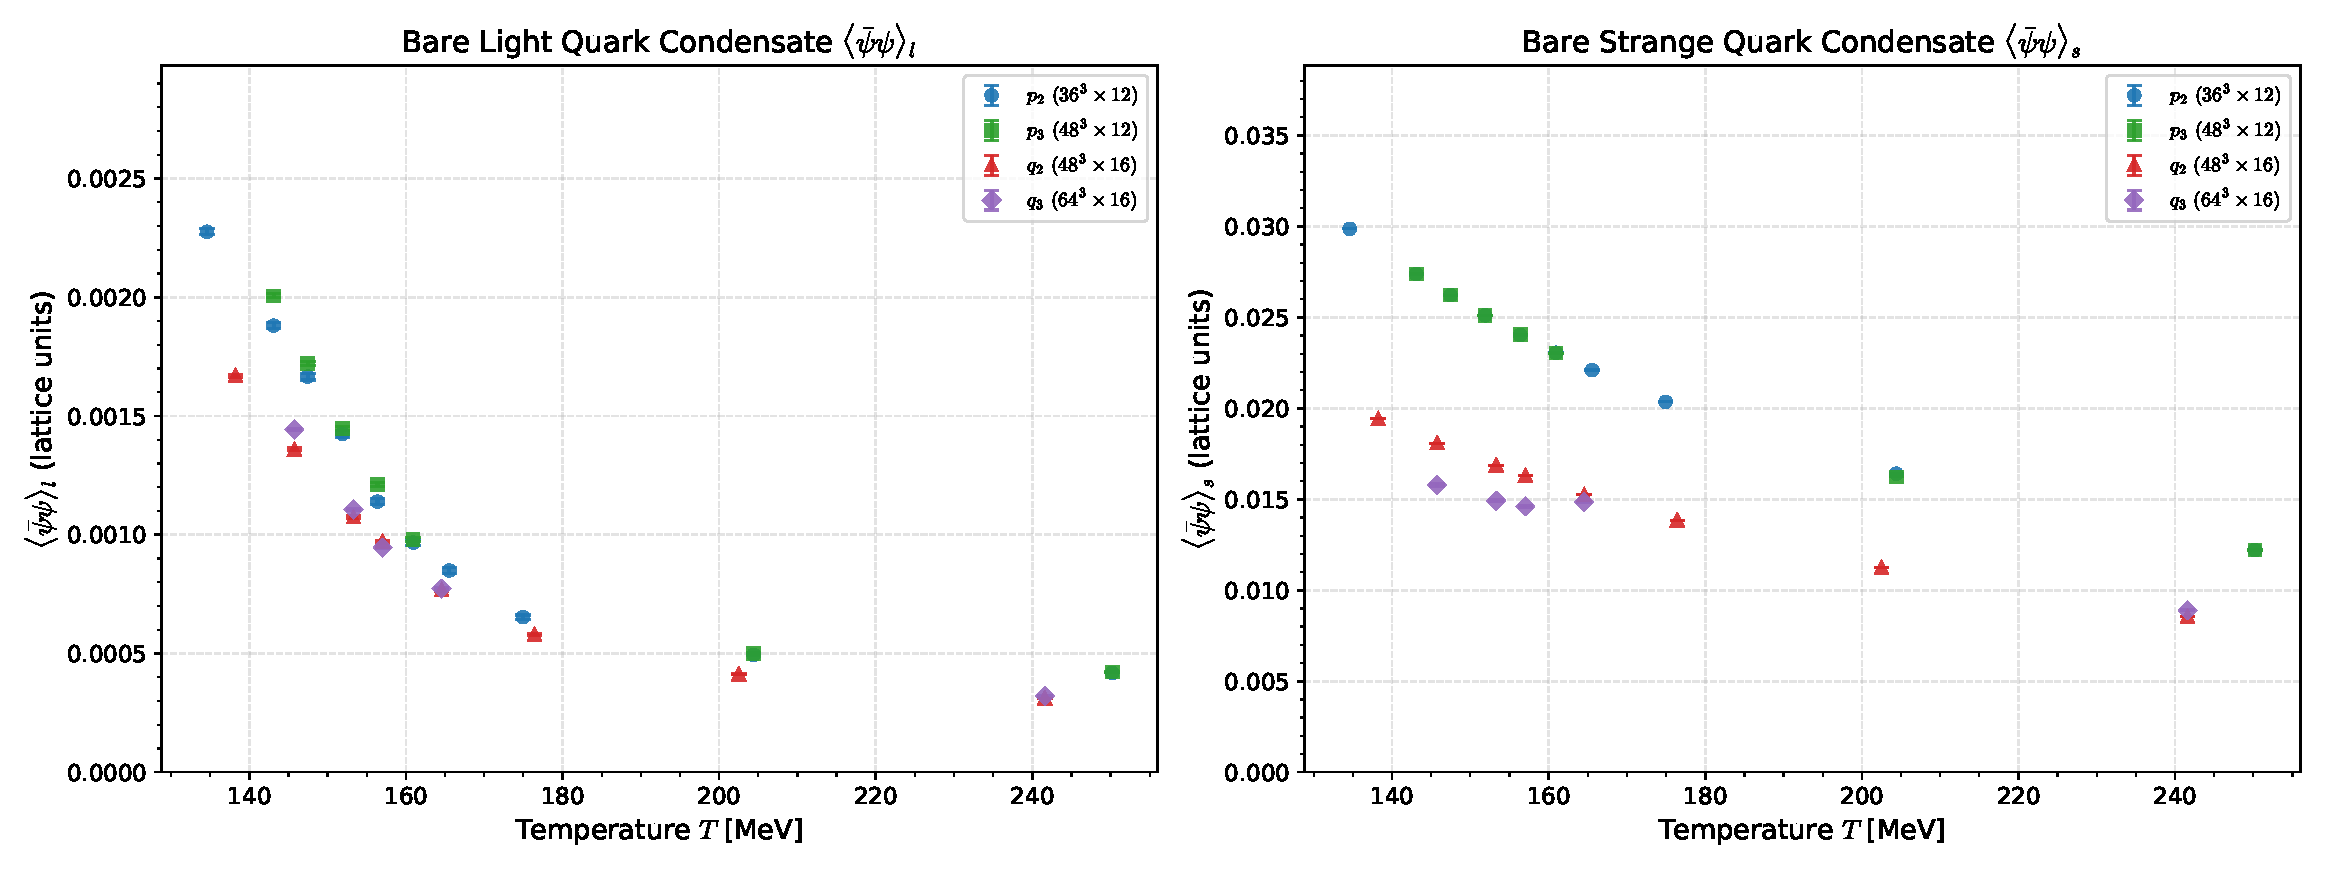
\includegraphics[width=\textwidth]{figures/chiral_condensate_bare_light_strange.pdf}
    \caption{Bare light quark condensate $\langle\bar{\psi}\psi\rangle_l$ (left) and bare strange quark condensate $\langle\bar{\psi}\psi\rangle_s$ (right) in lattice units across all four LCP ensembles ($p_2, p_3, q_2, q_3$).}
    \label{fig:bare_light_strange}
\end{figure}

The hight of peak, value of susceptibility, varies with Volume size slowly. The number of data points in q3 ensemble maybe  not so much but it's clearly larger than other ensembles.


\clearpage

\begin{figure}[htbp]
    \centering
    \begin{subfigure}[b]{0.49\textwidth}
        \centering
        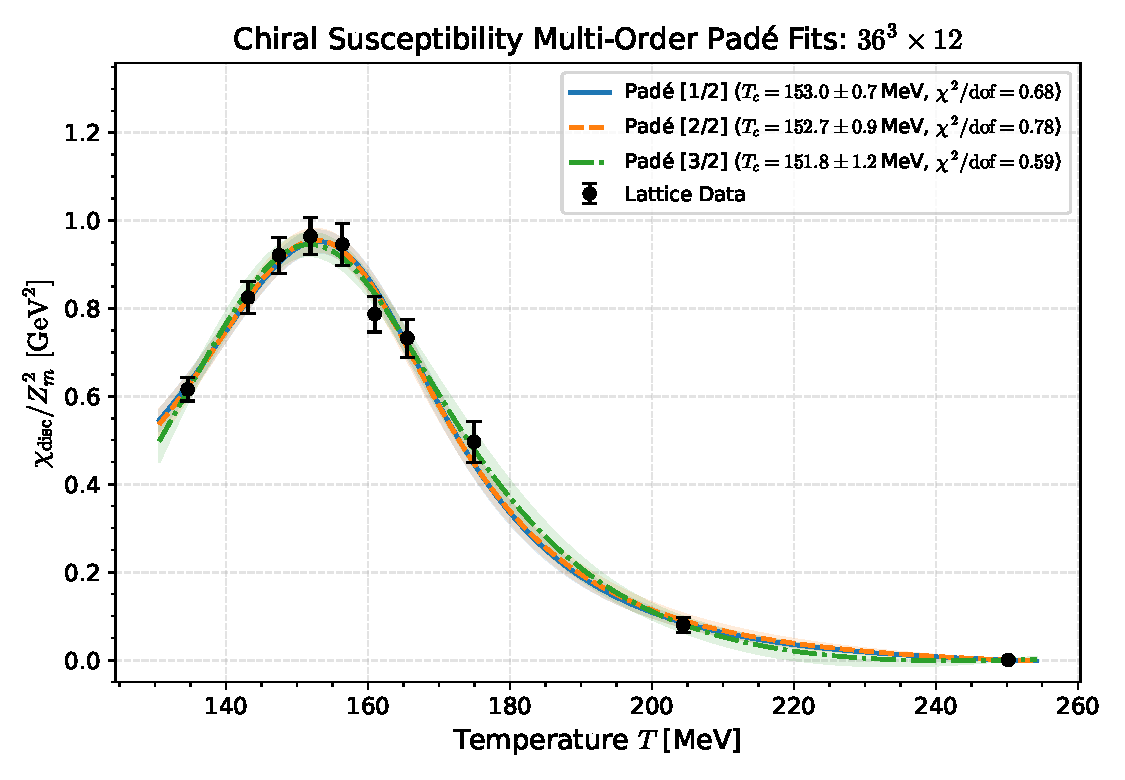
\includegraphics[width=\textwidth]{figures/chiral_susceptibility_multimodal_p2.pdf}
        \caption{$p_2$ ($36^3\times 12$)}
        \label{fig:multi_p2}
    \end{subfigure}
    \hfill
    \begin{subfigure}[b]{0.49\textwidth}
        \centering
        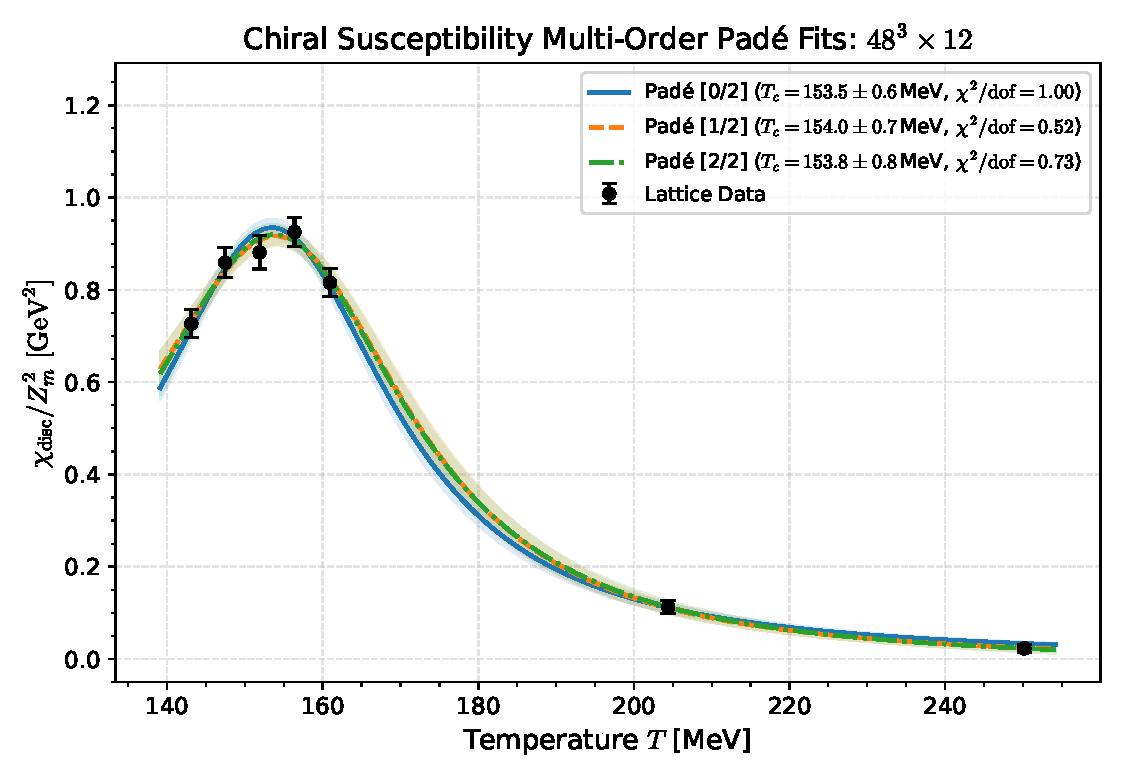
\includegraphics[width=\textwidth]{figures/chiral_susceptibility_multimodal_p3.pdf}
        \caption{$p_3$ ($48^3\times 12$)}
        \label{fig:multi_p3}
    \end{subfigure}
    \vskip\baselineskip
    \begin{subfigure}[b]{0.49\textwidth}
        \centering
        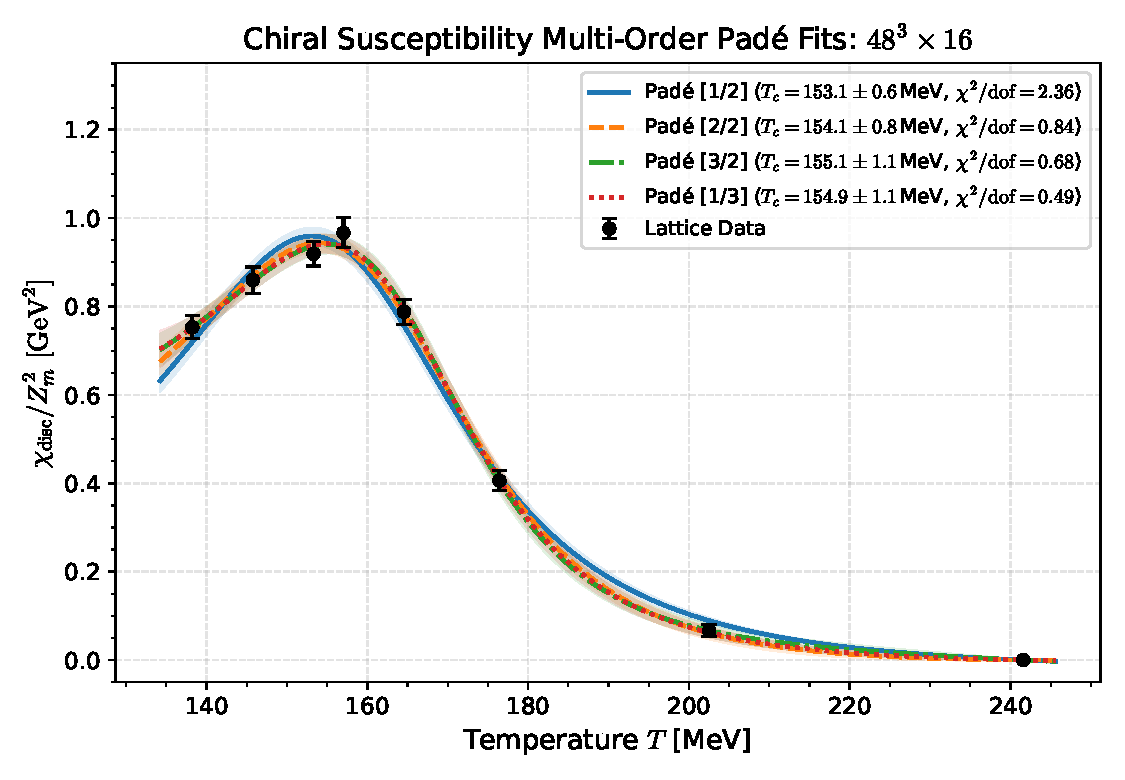
\includegraphics[width=\textwidth]{figures/chiral_susceptibility_multimodal_q2.pdf}
        \caption{$q_2$ ($48^3\times 16$)}
        \label{fig:multi_q2}
    \end{subfigure}
    \hfill
    \begin{subfigure}[b]{0.49\textwidth}
        \centering
        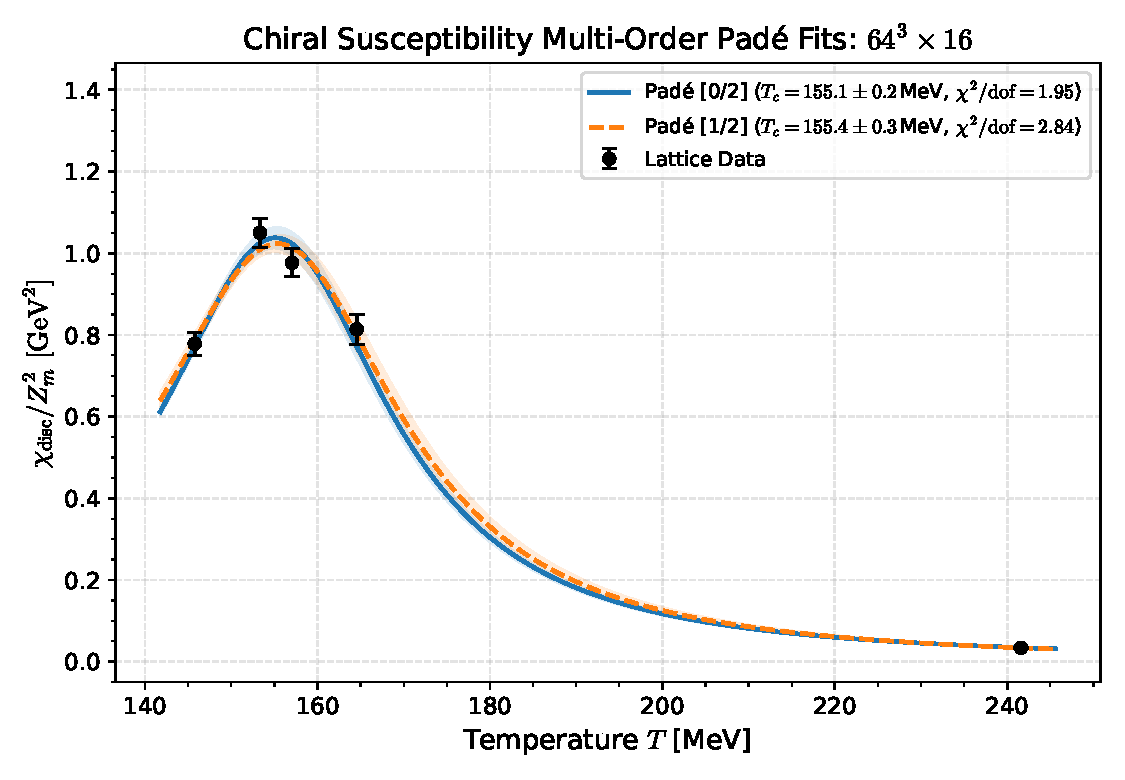
\includegraphics[width=\textwidth]{figures/chiral_susceptibility_multimodal_q3.pdf}
        \caption{$q_3$ ($64^3\times 16$)}
        \label{fig:multi_q3}
    \end{subfigure}
    \caption{Multi-order Padé approximation comparison per ensemble with shaded Jackknife confidence bands. }
    \label{fig:multimodal_all}
\end{figure}
Spurious orders suffering from real-axis poles or zero degrees of freedom have been excluded.

I picked the order with reduced chi2 close to 1, but the number of parameter, k, is also important.

\clearpage

\begin{table}[htbp]
    \centering
    \caption{Jackknife fit parameters and thermal transition results for primary Padé configurations.}
    \label{tab:lcp_summary}
    \small
    \begin{tabular}{lccccc}
        \toprule
        \textbf{Ensemble} & \textbf{Dimensions} & \textbf{Order} & $\boldsymbol{T_{pc}}$ [MeV] & $\boldsymbol{\chi_{\mathrm{peak}} / Z_m^2}$ [$\text{GeV}^2$] & $\boldsymbol{\chi^2/\mathrm{dof}}$ \\
        \midrule

        $p_{2}$ & $36^3\times 12$ & [2/2] & $152.74\pm 0.89$ & $0.956\pm 0.025$ & $0.775$ \\
        $p_{3}$ & $48^3\times 12$ & [0/2] & $153.48\pm 0.57$ & $0.935\pm 0.018$ & $1.000$ \\
        $q_{2}$ & $48^3\times 16$ & [2/2] & $154.06\pm 0.75$ & $0.944\pm 0.019$ & $0.840$ \\
        $q_{3}$ & $64^3\times 16$ & [0/2] & $155.12\pm 0.18$ & $1.038\pm 0.025$ & $1.952$ \\
        \bottomrule
    \end{tabular}
\end{table}

\begin{table}[htbp]
    \centering
    \caption{Model comparison across all Padé rational approximations.}
    \label{tab:model_comparison}
    \small
    \begin{tabular}{lcccc}
        \toprule
        \textbf{Ensemble} & \textbf{Order} & $\boldsymbol{k}$ & $\boldsymbol{\chi^2/\mathrm{dof}}$ & $\boldsymbol{T_{\mathrm{peak}}}$ [MeV] \\
        \midrule

        $p_{2}$ & [1/2] & 4 & $0.676$ & $152.99$ \\
        $p_{2}$ & [2/2] & 5 & $0.775$ & $152.74$ \\
        $p_{2}$ & [3/2] & 6 & $0.591$ & $151.79$ \\
        $p_{3}$ & [0/2] & 3 & $1.000$ & $153.48$ \\
        $p_{3}$ & [1/2] & 4 & $0.522$ & $153.98$ \\
        $p_{3}$ & [2/2] & 5 & $0.728$ & $153.82$ \\
        $q_{2}$ & [1/2] & 4 & $2.357$ & $153.07$ \\
        $q_{2}$ & [2/2] & 5 & $0.840$ & $154.06$ \\
        $q_{2}$ & [3/2] & 6 & $0.675$ & $155.11$ \\
        $q_{2}$ & [1/3] & 5 & $0.492$ & $154.92$ \\
        $q_{3}$ & [0/2] & 3 & $1.952$ & $155.12$ \\
        $q_{3}$ & [1/2] & 4 & $2.843$ & $155.39$ \\
        \bottomrule
    \end{tabular}
\end{table}

\clearpage

\begin{table}[htbp]
    \centering
    \caption{Lattice measurements for $N_t=12$ ensembles ($p_2$ and $p_3$): Temperature $T$, inverse lattice spacing $a^{-1}$, renormalized chiral condensate $\langle\bar{\psi}\psi\rangle_{\mathrm{sub}}/Z_m$ in lattice units, and renormalized susceptibility $\chi_{\mathrm{disc}} / Z_m^2$ [$\text{GeV}^2$].}
    \label{tab:raw_p2_p3}
    \small
    \begin{tabular}{lccccc}
        \toprule
        \textbf{Ensemble} & $\boldsymbol{\beta}$ & $\boldsymbol{T}$ [MeV] & $\boldsymbol{a^{-1}}$ [GeV] & $\boldsymbol{\langle\bar{\psi}\psi\rangle_{\mathrm{sub}}/Z_m}$ & $\boldsymbol{\chi_{\mathrm{disc}} / Z_m^2}$ [$\text{GeV}^2$] \\
        \midrule

        $p_2$ ($36^3\times 12$) & 4.020 & 134.6 & 1.615 & $(1.36 \pm 0.01) \times 10^{-3}$ & $(6.158 \pm 0.262) \times 10^{-1}$ \\
        $p_2$ ($36^3\times 12$) & 4.040 & 143.1 & 1.717 & $(9.70 \pm 0.16) \times 10^{-4}$ & $(8.249 \pm 0.364) \times 10^{-1}$ \\
        $p_2$ ($36^3\times 12$) & 4.050 & 147.5 & 1.770 & $(7.76 \pm 0.16) \times 10^{-4}$ & $(9.208 \pm 0.416) \times 10^{-1}$ \\
        $p_2$ ($36^3\times 12$) & 4.060 & 151.9 & 1.823 & $(5.51 \pm 0.16) \times 10^{-4}$ & $(9.644 \pm 0.419) \times 10^{-1}$ \\
        $p_2$ ($36^3\times 12$) & 4.070 & 156.4 & 1.877 & $(2.83 \pm 0.15) \times 10^{-4}$ & $(9.459 \pm 0.481) \times 10^{-1}$ \\
        $p_2$ ($36^3\times 12$) & 4.080 & 160.9 & 1.931 & $(1.38 \pm 0.14) \times 10^{-4}$ & $(7.872 \pm 0.407) \times 10^{-1}$ \\
        $p_2$ ($36^3\times 12$) & 4.090 & 165.5 & 1.986 & $(5.23 \pm 1.29) \times 10^{-5}$ & $(7.326 \pm 0.432) \times 10^{-1}$ \\
        $p_2$ ($36^3\times 12$) & 4.110 & 174.9 & 2.099 & $(-6.88 \pm 1.00) \times 10^{-5}$ & $(4.964 \pm 0.463) \times 10^{-1}$ \\
        $p_2$ ($36^3\times 12$) & 4.170 & 204.4 & 2.453 & $(-7.00 \pm 0.35) \times 10^{-5}$ & $(8.000 \pm 1.651) \times 10^{-2}$ \\
        $p_2$ ($36^3\times 12$) & 4.260 & 250.2 & 3.002 & $(-1.48 \pm 0.02) \times 10^{-5}$ & $(3.595 \pm 0.816) \times 10^{-4}$ \\
        \midrule

        $p_3$ ($48^3\times 12$) & 4.040 & 143.1 & 1.717 & $(1.12 \pm 0.01) \times 10^{-3}$ & $(7.266 \pm 0.299) \times 10^{-1}$ \\
        $p_3$ ($48^3\times 12$) & 4.050 & 147.5 & 1.770 & $(8.41 \pm 0.10) \times 10^{-4}$ & $(8.592 \pm 0.330) \times 10^{-1}$ \\
        $p_3$ ($48^3\times 12$) & 4.060 & 151.9 & 1.823 & $(5.78 \pm 0.10) \times 10^{-4}$ & $(8.810 \pm 0.358) \times 10^{-1}$ \\
        $p_3$ ($48^3\times 12$) & 4.070 & 156.4 & 1.877 & $(3.65 \pm 0.10) \times 10^{-4}$ & $(9.254 \pm 0.313) \times 10^{-1}$ \\
        $p_3$ ($48^3\times 12$) & 4.080 & 160.9 & 1.931 & $(1.54 \pm 0.09) \times 10^{-4}$ & $(8.157 \pm 0.298) \times 10^{-1}$ \\
        $p_3$ ($48^3\times 12$) & 4.170 & 204.4 & 2.453 & $(-6.42 \pm 0.27) \times 10^{-5}$ & $(1.131 \pm 0.133) \times 10^{-1}$ \\
        $p_3$ ($48^3\times 12$) & 4.260 & 250.2 & 3.002 & $(-1.17 \pm 0.09) \times 10^{-5}$ & $(2.301 \pm 0.817) \times 10^{-2}$ \\
        \bottomrule
    \end{tabular}
\end{table}

\begin{table}[htbp]
    \centering
    \caption{Lattice measurements for $N_t=16$ ensembles ($q_2$ and $q_3$): Temperature $T$, inverse lattice spacing $a^{-1}$, renormalized chiral condensate $\langle\bar{\psi}\psi\rangle_{\mathrm{sub}}/Z_m$ in lattice units, and renormalized susceptibility $\chi_{\mathrm{disc}} / Z_m^2$ [$\text{GeV}^2$].}
    \label{tab:raw_q2_q3}
    \small
    \begin{tabular}{lccccc}
        \toprule
        \textbf{Ensemble} & $\boldsymbol{\beta}$ & $\boldsymbol{T}$ [MeV] & $\boldsymbol{a^{-1}}$ [GeV] & $\boldsymbol{\langle\bar{\psi}\psi\rangle_{\mathrm{sub}}/Z_m}$ & $\boldsymbol{\chi_{\mathrm{disc}} / Z_m^2}$ [$\text{GeV}^2$] \\
        \midrule

        $q_2$ ($48^3\times 16$) & 4.130 & 138.2 & 2.212 & $(1.13 \pm 0.01) \times 10^{-3}$ & $(7.531 \pm 0.262) \times 10^{-1}$ \\
        $q_2$ ($48^3\times 16$) & 4.150 & 145.8 & 2.332 & $(8.10 \pm 0.07) \times 10^{-4}$ & $(8.600 \pm 0.295) \times 10^{-1}$ \\
        $q_2$ ($48^3\times 16$) & 4.170 & 153.3 & 2.453 & $(5.25 \pm 0.07) \times 10^{-4}$ & $(9.193 \pm 0.276) \times 10^{-1}$ \\
        $q_2$ ($48^3\times 16$) & 4.180 & 157.0 & 2.512 & $(4.28 \pm 0.07) \times 10^{-4}$ & $(9.666 \pm 0.341) \times 10^{-1}$ \\
        $q_2$ ($48^3\times 16$) & 4.200 & 164.6 & 2.633 & $(2.42 \pm 0.06) \times 10^{-4}$ & $(7.883 \pm 0.285) \times 10^{-1}$ \\
        $q_2$ ($48^3\times 16$) & 4.230 & 176.4 & 2.823 & $(9.25 \pm 0.38) \times 10^{-5}$ & $(4.059 \pm 0.230) \times 10^{-1}$ \\
        $q_2$ ($48^3\times 16$) & 4.300 & 202.5 & 3.240 & $(7.87 \pm 1.27) \times 10^{-6}$ & $(6.621 \pm 1.383) \times 10^{-2}$ \\
        $q_2$ ($48^3\times 16$) & 4.405 & 241.6 & 3.866 & $(3.69 \pm 0.19) \times 10^{-7}$ & $(7.244 \pm 1.418) \times 10^{-5}$ \\
        \midrule

        $q_3$ ($64^3\times 16$) & 4.150 & 145.8 & 2.332 & $(9.89 \pm 0.05) \times 10^{-4}$ & $(7.784 \pm 0.279) \times 10^{-1}$ \\
        $q_3$ ($64^3\times 16$) & 4.170 & 153.3 & 2.453 & $(6.32 \pm 0.05) \times 10^{-4}$ & $1.050 \pm 0.035$ \\
        $q_3$ ($64^3\times 16$) & 4.180 & 157.0 & 2.512 & $(4.63 \pm 0.05) \times 10^{-4}$ & $(9.766 \pm 0.339) \times 10^{-1}$ \\
        $q_3$ ($64^3\times 16$) & 4.200 & 164.6 & 2.633 & $(2.62 \pm 0.05) \times 10^{-4}$ & $(8.137 \pm 0.369) \times 10^{-1}$ \\
        $q_3$ ($64^3\times 16$) & 4.405 & 241.6 & 3.866 & $(-1.12 \pm 0.09) \times 10^{-6}$ & $(3.396 \pm 0.157) \times 10^{-2}$ \\
        \bottomrule
    \end{tabular}
\end{table}

\end{document}
